\chapter[OLD Model Implementation]{OLD Model Implementation}
\label{appendix-model-implementation}

% \section{Urban wage premium}

% $\omega$ is the urban wage premium. It is a share of the urban agglomeration effect. 

% I think of this as worker income, $\psi + \omega + r_prime*savings$ 

% The wage income  $\psi + \omega$ part has to be related to the marginal productivity of workers. The urban output function from Lobo et al \cite{loboUrbanScalingProduction2013} is  
% \begin{equation}Y=AN^\beta\label{LoboEqn2}\end{equation}

% Where $\beta$  is the scaling exponent, with a value of,  for example, 1.13  \`a la 
% Lobo. $A$ is called the ``scale factor.''\footnote{Much of the analysis assumes scale invariance of  $A$.}  The \textbf{total urban marginal productivity of a worker} is  
% \[UMPL=\beta AN^{\beta-1}=\frac{\beta Y}{N} =\]
% This is not the same as the \textbf{firm-level marginal productivity of a worker}. The worker total share in Lobo et al. is \[W= (1-\alpha)Y \] 
% so the individual share, which should be the competitive wage, is
% \[W= \frac{(1-\alpha)Y}{N} \] 
% where $(1-\alpha)=0.8$ is a common estimate. If we assume that this sets the rural wage,$\phi$, then $\omega$ has to come out of the  urban surplus per worker,

% \[surp= \frac{\beta -(1-\alpha)Y}{N} \] 

%  so set a fraction $\lambda$ of the surplus a, and 
%  \[\omega= \lambda\frac{\beta -(1-\alpha)Y}{N}= (1.13-.8) \frac{Y}{N} \] 


% $(\beta -1)$ is agglom and  $\lambda(\beta -1)$ is the workers' share of the surplus over and above the \gls{constant returns to scale} (CRS) case.   $\lambda(\beta -1)$ is 


{\color{orange} THIS BLOCK HAS BEEN MOVED TO APPENDIX 3 ON PARAMETERS

\section{Wage calculation}
Firms make two decisions faced with a market wage. They hire and they adjust their wage. This is typical in \glspl{competitive market} where firms are price-takers. They do not make  wage offers in this model. That happens when firms have a degree of market power.)


When aggregate firm labour demand exceeds N, wages rise 
% Common to think of the variations in local wages as variations around a mean, in this context - perfect labour market.
% We're using this number at the agregate level, raise the market wage to a level that attracts that many. Divide available workers among the firms, then they want to raise the wage again. It's more transparent to do it at the agregate level than at the firm level, but we still have the rising supply curve. A more detailed agent model could implement the hiring and wage adjustment mechanisms for firms dirrectly, but the side effect of increased ocmplication is it also can obscure the clarity of the rent results, our focus wit this work. 
\begin{lstlisting}
# TODO FIX TOTALY - MOVE THIS TO THE MODEL SECTION NOW #
# Firm step function updates wage, omega
def step(self):
    prefactor  = self.model.prefactor
    agglom     = self.model.agglomeration_ratio
    population = self.model.agglomeration_population
    wage_share = self.model.wage_share  
    wage_premium = wage_share * (agglom-1) * prefactor * population**agglom # omega # ****** 
    self.wage = wage_premium + self.model.psi
    # k thought # self.wage_premium = (wage_share * prefactor * population**agglom)/ population # omega    
    # note surplus is: (beta - 1) * (prefactor * population**agglom)
\end{lstlisting}

Where wage share is a parameter input to the model.

\section{Bidding}
\subsection{Subjective discounting}

The discount factor gives the present value of one dollar received at particular point in the future, given the date of receipt and the discount rate.

% growth rate= rt
% growth factor =($1+r)^t$
% discount rate= r
% discount factor = $1/(1+r)^t$
    
\begin{lstlisting}
def get_discount_factor(self):
    """
    The discount factor gives the present value of one dollar received at particular point in the future, given the date of receipt and the discount rate.
    Delta is the subjective individual discount rate for agent
    after one year. This will be close to the prime interest rate, r_i.
    """    
    delta = self.r_prime
    delta_period_1 = 1 / (1 + delta) 
    delta_mortgage_period = delta_period_1**self.mortgage_period
    sum_delta = (1 - delta_mortgage_period)/delta
    return sum_delta
\end{lstlisting}
% #   sum_delta = delta_mortgage_period * (1 - delta_mortgage_period) # Old
Delta could als%o depend on wealth. For example,  use the bank rate, which is the rational rate but people who are poor typically have higher rates.  It would not change as the central bank changes r-pirme
% delta could be wealth based typically higher for poor.

% sum\_delta is sum of the infinite series minus discounted infinite series after mortgage\_period years
% Here, it is the present value of annual payments from one to mortgage\_period years e.g. of mortgage payments or rent received. 
% delta\_mortgage\_period was previously called   delta\_period\_T 
% # Note delta_mortgage_period is subtracted to subtract the long tail. 1/delta gives the PV of an infineite series of payments

\begin{lstlisting}
# A version with delta depending on wealth
wealth = self.wealth
delta =
\end{lstlisting}
% savings =(sum(0-age)((1+r)**age)*savings_rate*subsistence)

\subsection{Maintenance costs}
\begin{lstlisting}
def get_maintenance(self):
    """Maintenance share of property service (a*b*psi summed and discounted)
    OR IS IT TOTAL maintenance COST OVER THE MORTGAGE PERIOD?
    """
    a   = self.housing_services_share
    b   = self.maintenance_share
    psi = self.subsistence_wage
    sum_delta = self.sum_delta # CALCULATE PER PERSON
    return (a * b * psi) * sum_delta
\end{lstlisting}

\subsection{Taxes}
TODO Should taxes depend on wages? Maybe depend on the urban wage?
% THIS DOES NOT CHANGE WITH INCREASING WAGES?
% BUT THAT IS THE MAIN WAY TO FUND A CITY

% WHAT TO CALL THIS WEHRE DOES IT GO. WHERE DO WE USE THIS VS TAU
%         Just for initialization? - warranted price. 
%         Use warranted prices as initialization
%         Tax costs for the mortgage period, T. 
%         (Example of rate for an  multiperiod annual rate)
%         tax_T= tau*(omega-c*d + a*psi) * sum_delta_T
%         This is assuming taxes are paid at the end of each year for T years
%         tau_T       = tau * sum_T_delta 
%         #  present value of the tax rate over T years        
%         """

        
\begin{lstlisting}
    def get_tax(self):
        tau   = self.model.property_tax_annually
        omega = self.model.firm.wage_premium # FIXED
        psi   = self.model.subsistence_wage
        a     = self.model.housing_services_share
        c     = self.model.transport_cost_per_dist # RENAME
        d     = self.distance_from_center
        sum_delta = self.model.sum_delta # TODO - make individual  - this would have to be average discounting - THIS TAKE SUM DELTA OUT - AND PUT WITH LARGER CALCULATION.. - CACLULATE FOR A PERSON/PROPERTY COMBINATION..
        return tau * (omega - c*d + a*psi) * sum_delta
\end{lstlisting}


\subsection{TODO Warranted price}

TEMP
\begin{align*}
\mathcal{T} &= \text{mill rate} \times \frac{\mathcal{R}_W}{r} \\
&= c \times \frac{\omega- {dc} + a\psi.}{r}
\end{align*}

\begin{lstlisting}
@property
def warranted_price(self):
    omega = self.model.firm.wage_premium # FIXED
    psi   = self.model.subsistence_wage
    a     = self.model.housing_services_share
    c     = self.model.transport_cost_per_dist # RENAME
    d     = self.distance_from_center
    r     = self.model.prime # CHECK name
    return c * (omega - d*c + a*psi) / r
    
    # USELESS PLACEHOLDER - GET CALCULATION
    return self.model.firm.wage/(self.transport_cost + 1) 
\end{lstlisting}


\subsection{TODO Maximum bid price}

Agents compute their maximum bid, and the negotiation process adjusts downwards as appropriate REF.

\begin{eqnarray}
P_B^{max} & \le    \frac{\mathcal{R}_N}{(1-m)r^{target}-\delta \left(1 + \dot P_M^e - (1+r)m\right)} \label{eqn-bid-price} \end{eqnarray}

In banking with individual information on a land parcel and person.
\begin{lstlisting}
def get_max_bid_price(self, bidder, property):
    net_rent = property.get_net_rent()
    m        = bidder.get_max_mortgage()
    r        = self.model.sum_r # SAME AS SUM_R? RENAME?
    r_target = r_prime + agents_premium # FIX
    delta    = self.model.sum_delta # SAME AS SUM_DELTA? RENAME?
    P_dot    = GET FROM THE CURVE FIT
    denominator = (1-m)*r_target - delta*(1 + P_dot  - (1+r)*m)
    return net_rent / denominator   
\end{lstlisting}

\textbf{TODO FIX - little m is the max someone qualifies for.. we also have a maximum amount. Need to reconcile those two approaches.}
 
\subsection{TODO Maximum mortgage calculation}

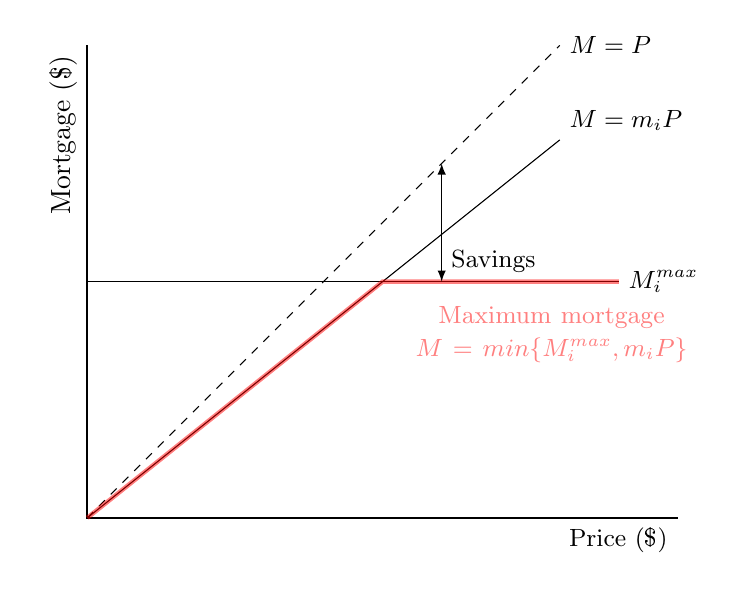
\begin{tikzpicture}	[scale=1.5]
\draw[thick] (0,4)node[above left, align = center,rotate=90]{\small \\Mortgage (\$)} --(0,0)--(5,0)node[below left]{\small Price (\$)}; 
\draw[dashed] (0,0)--(4,4)node[right]{\small $M=P$};
\draw[] (0,2)--(4.5,2)node[right]{\small $M_i^{max}$};
\draw[] (0,0)--(4,3.2)node[above right]{\small $M=m_iP$};
\draw[ultra thick, red, opacity=.5] (0,0)--(2.5,2)node[below right,  text width=4cm, align = center]{\small \\ Maximum mortgage \\ $M=min\{M_i^{max}, m_iP\}$}--(4.5,2);
\draw[latex-latex] (3,2)node[above right] {\small Savings}--(3,3);
\end{tikzpicture}

Mortgage gives 2 numbers. First it pays for a share of the purchase price, second it has an actual maximum. There's a line with a kink because there's 2 constraints.  The difference between the two diagonal lines is what you pay from savings. 
The diagonal line - the top dashed diagonal line is just the line where the mortgage would be price.
% This is just the constraint. Up to the kink, little $m_i$ is a fraction of price. beyond rhtat little mi becomes a different number - number based on little $m_i$ for everyone
% banks have an advantage since they can practically bid anything
% m - mortgage share
% P - realized price
% M - maximum - 

\textbf{Wealth-based mortgage maximum} 
 \[max\ m_i = 9-\left(\frac{W_i}{\bar W}\right)^{0.1} \]

% **Source**: Ch:model line 580, page 87.. I have done some fiddling Wealth $W_i = P-M+S.  for i - real estate agents estimated price wealth of a property owner as assessed by the bank

\textbf{Income-based mortgage maximum}

\[M^{max}_Yi = \frac{0.28*(\psi + \omega)}{r_i}\] It is the maximum the bank will let you pay.  0.28 is a parameter {ability to carry a mortgage}.
 
\textbf{Combined mortgage maximum}
\[ M_i^{max} = min \{9-\left(\frac{W_i}{\bar W}\right)^{0.1}P,  \frac{0.28*(\psi + \omega)}{r_i} \}\]
Because we use $m_i$ in calculating the maximum bid for individuals and it in effect changes after the inflection point in the graph, we need some adjustments. 

First, the maximum price that will be offered is the minimum of $M^{max_i} +S$ and the maximum bid calculated using $m_i$ (which is calculated independently) if 
$P\le \frac{M_i^{max}}{m_i}$ 
and $m_i^*$ if 
$P\ge \frac{M_i^{max}}{m_i}$, where 
\[m_i^*=\frac{M_i^{max}}{P}\]

\begin{lstlisting}
# parameters - max interest payment 
ability_to_carry_mortgage = .28 # ability to cover a mortgage OR 9?
max_mortgage_share = 0.9
WHAT IS 0.1?

# Agents initialize wealth and update in each step ..
# set newcomer property_value and mortgage size to 0

def get_max_mortgage(self, applicant):
    wealth = applicant.wealth
    mean_wealth = self.model.mean_wealth
    wealth_max = applicant.max_mortgage_share - (wealth/mean_wealth)**
mean_weath = sum(wealth)/number_of_people

def get_max_mortgage(self, applicant):
    max_mortgage =  ...
    
    return max_mortgage
\end{lstlisting}

% wealth = property_value + 
wealth $W_i = P_e-M+S$.  

- Also need mean wealth. $\bar W$ , which you have to calculate from the sums for property values total mortgages issued, and individual savings. The bank could keep these values

- Individual borrowing rate 
$r_i = (A + B \frac{\bar{W}}{W_i})\bar r=(.1 + B \frac{\bar{W}}{W_i})\bar r$.
The value .1 can be seen as the bank's share of the prime rate set by the Bank of Canada. this is an easy place to insert that value. We should discuss this detail. An alternative is
$r_i = (0 + B \frac{\bar{W}}{W_i})(\bar r_i+ bank\ margin)$.

- Maximum M  from wealth constraint = $(9-(W_i/\bar W)^{0.1}P$

where 9 is the maximum mortgage share. (SHOULD IT BE 0.9?)

  Check if $(W_i/\bar W)0.9P$ will work. 


END OF TRANSFERRED BLOCK
}

- Maximum M  from income = $M^{max}_Yi = \frac{0.28*(\omega+w)}{r_i}$ 
% - Maximum M  $M= min(0.28*(omega+phi)/r_i,  0.8P$,  (9-(W_i/\bar W)^{0.1}P,  \frac{0.28*(\omega+w)}{r_i}   } $
 
\subsection{Net rent based on}
Tenant willing to pay, vs what it is worth for a company to buy a property.


CHECKED - PUT CHANGE BACK IN CODE.

\begin{lstlisting}
def get_net_rent(self, property):
    """Compute the rent for a land parcel, or what someone could afford
    to pay to live there. 

    Rent depends on the urban wage premium over and above the subsistence
    wage, and on transportation costs and the distance to the
    central business district. Applies with a single wage. Adjust for
    differential urban wages.

    :param property: the land parcel to get rent information for.
    """
    a     = self.model.housing_services_share
    b     = self.model.maintenance_share
    c     = self.model.transport_cost_per_dist # RENAME
    d     = property.distance_from_center 
    tau   = self.model.property_tax_annually 
    # property_tax_rate # IS THIS FOR THE MORTGAGE PERIOD
    psi   = self.model.subsistence_wage
    omega = self.model.firm.wage_premium 
    return omega - c*d - a*psi - b*a*psi - tau*a*psi
    # urban_wage = self.model.firm.wage
\end{lstlisting}


\subsection{Net rent based on ..}

REPETITION - CUT
% \begin{lstlisting}
% def get_net_rent(self, property):
%     """Compute the rent for a land parcel, or what someone could afford
%     to pay to live there. 

%     Rent depends on the urban wage premium over and above the subsistence
%     wage, and on transportation costs and the distance to the
%     central business district. Applies with a single wage. Adjust for
%     differential urban wages.

%     :param property: the land parcel to get rent information for.
%     """
%     a     = self.model.housing_services_share
%     b     = self.model.maintenance_share
%     c     = self.model.transport_cost_per_dist # RENAME
%     d     = property.distance_from_center 
%     tau   = self.model.property_tax_annually 
%     # property_tax_rate # IS THIS FOR THE MORTGAGE PERIOD
%     psi   = self.model.subsistence_wage
%     omega = WAGE_PREMIUM self.model.workers_share
%     return omega - c*d - a*psi - b*a*psi - tau*a*psi
%     # urban_wage = self.model.firm.wage
% \end{lstlisting}

\subsection{Max bid}

Calculate max desired bid for an agent
\begin{lstlisting}
    def get_max_bid(self, property, bidder):
        net_rent  = self.get_net_rent(property)
        r         = self.model.r_prime   
        r_target  = r + self.model.r_premium
        m         = 0.8 # TODO FIX - ADD WEALTH
        # I can't do delta_T. It reads as delta_transpose to me.
        sum_delta = self.model.sum_delta 
        p_dot     = 0.01 # TODO - estimate rate of price change
        return net_rent/((1 - m)*r_target - sum_delta*(1 + p_dot - (1 + r)*m))
\end{lstlisting}

Agent will bid the min of the desired bid or the max allowed mortgage
\begin{lstlisting}
max_mortgage = self.bank.get_max_mortgage(self)
min_downpayment = self.bank.min_down_payment_share * max_mortgage
downpayment = min(min_downpayment, self.savings)
max_allowed_bid = max_mortgage + downpayment
for sale_property in (self.model.realtor.sale_listing):
    # max_bid = self.bank.get_max_bid(sale_property, self)
    # TODO Fix
    max_desired_bid = self.model.bank.get_max_bid(sale_property, self)
    max_bid = min(max_allowed_bid, max_desired_bid)
\end{lstlisting}

\section{Negotiation Process}

Bidding.

There is a problem in that they bid on all properties as a shortcut. If the number of bids structures the negotiation process, we need to limit their bids or do something much more iterative. (see above section)


\section{Individual Accounting}
UPDATE CODE
GET prime interest rate - R
\begin{lstlisting}
# FIX - NEED TO ADD THIS
# Update savings

self.savings += self.model.savings_per_step + r*self.savings

# TODO pay costs for any properties owned
# if self.residence in self.properties_owned:
#     # TODO pay mortgage if needed pay costs
#     pass
# else:
#     self.savings -= self.rent # TODO check this is right rent
\end{lstlisting}